% !TEX root = ../thesis.tex
% -------------------------------------------------------------
\subsubsection{Variational inference in the exponential family}
%
The premises of both ADF and EP is performing variational inference in the exponential family $\mathcal F_{\phi}(\mathcal X)$.\add{check EP/ADF introduced} In the previous point, we showed that a target distribution $p$ could be associated with a point $\mu_p\in\mathcal M$ with $\mu_p=\E_{p}[\phi(X)]$ for a sufficient statistic $\phi$. Further, we showed that if the family is minimal and if $\mu_p\in\mathcal M^{\star}$, the mean parameter could be directly associated to a distribution in $\mathcal F_{\phi}(\mathcal X)$ with parameter $\theta$ given by $\nabla A^{\star}(\mu_p)$. It is therefore natural to consider this distribution $q_{\theta}$ as potentially forming a good approximation to $p$ in $\mathcal F_{\phi}(\mathcal X)$.\check{may15,april24}
%
%\begin{figure}[!h]
%    \center
%	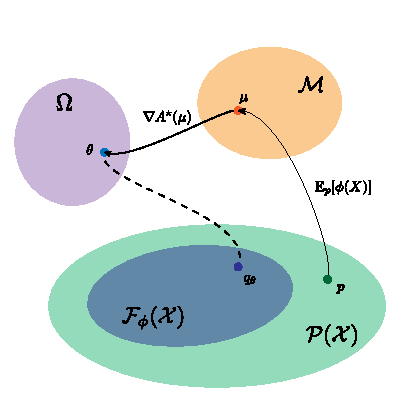
\includegraphics[width=.5\textwidth]{figures/expf/mapping2}
%\caption{blah}
%\end{figure}
This is supported by the fact that this distribution actually minimises the divergence $\KL{p,q_{\theta'}}$. Indeed, observe that
%
\eqa{
	\KL{p,q_{\theta'}} &=& \E_{p}[\log p] - \scal{\theta', \mu_p} + A(\theta'), \label{kldivadf}
}
%
which is a strictly convex function in $\theta'$. By definition, a parameter $\theta=\nabla A^{\star}(\mu_p)$ is such that $\nabla A(\theta)=\mu_p$ and therefore verifies the first order condition. This shows that $q_{\theta}$ minimises the divergence \eqref{kldivadf}. It is useful at this point to define a projection operator $\mathbf P_{\phi}:\mathcal P(\mathcal X) \to \mathrm{cl}(\Omega)$\, with
%
\eqa{	
	\theta \,\,=\,\, \mathbf P_{\phi}[p] &\Longleftrightarrow& \theta \,\,=\,\, \nabla A^{\star}(\E_{p}[\phi(X)]).
}
%
Assuming $\mathbf P_{\phi}[p] \in \Omega$, $q_{\theta}$ is a proper distribution in $\mathcal F_{\phi}(\mathcal X)$ that minimises the KL \eqref{kldivadf} and equivalently verifies the \emph{global moment matching condition} (GMMC) 
%
\eqa{
	(\text{GMMC})\qquad \E_{q_{\theta}}[\phi(X)]&=&\E_{p}[\phi(X)].
\label{eq:GMMC}}
%
It will also be convenient to use the following abuse of notation: for an unnormalised distribution $p_{u}$ with some normalisation constant $Z_{p_{u}}\inv$ we will write $\mathbf P_{\phi}[p_{u}]$ to implicitly mean $\mathbf P_{\phi}[Z_{p_{u}}\inv p_{u}]$.\check{may15,april24}

The application of this projection operator implicitly requires the ability to perform two computations. First, it requires the ability to compute the expected value $\mu_p=\E_{p}[\phi(X)]$ which is typically intractable since we are in a context where we are trying to approximate $p$ for that very purpose. Then, provided we can compute $\mu_p$, we need to be able to apply the inverse mapping $\nabla A^{\star}(\mu_p)$. We will introduce below contexts in which the first requirement can be approximately met. The second requirement effectively means that we are constrained to exponential families for which computing the inverse mapping $\nabla A^{\star}$ can be done explicitly or is cheap to approximate. For continuous state spaces, it is overwhelmingly the Gaussian distribution that is considered in the literature with either a diagonal or a full covariance matrix.\add{probably add a section here on how to compute forward backward operator, maybe put this in appendix. Also cite lots of stuff that uses the Gaussian, if you find anything that doesn't...}\check{may15,april24} 
%
% ----------------------------------------
\subsubsection*{Online Bayesian Learning and Assumed Density Filtering}
%
Let us consider the context of online Bayesian learning where one is interested in the evolution of a posterior distribution $p(x\st y_{1:t})$ given observed \iid\add{notations iid} data points $y_{1:t}$ up to current time $t$ and a new \iid data point $y_{t+1}$. The new posterior is given directly by Bayes rule with $p(x\st y_{1:t+1})\propto p(y_{t+1}\st x) p(x\st y_{1:t})$. In \citet{opper98}, the author considers that the exact posteriors are intractable but suggests constructing a sequence of approximations in the exponential family $\mathcal F_{\phi}(\mathcal X)$. Using the notations from the previous point, the algorithm corresponds to a sequence of iteration of the form
\eqa{	\theta_{t+1} &=& \mathbf P_{\phi}[p(y_{t+1}\st \cdot)q_{\theta_{t}}],	\label{adfonline}}
where, at the first step, $q_{\theta_{0}}$ is replaced by the prior $\pi_{0}$. In words, the posterior up to time $t$ is approximated by the exponential family distribution $q_{\theta_{t}}$ which then serves as prior to form an approximate posterior $p(y_{t+1}\st x)q_{\theta_{t}}(x)$. Given that this approximate posterior is not necessarily in the exponential family, it needs to be projected as per \eqref{adfonline}.\check{april27} At time $t+1$, the distribution $q_{\theta_{t+1}}$ can be now interpreted as an approximation of the posterior distribution given all the data up to that time or 
%
\eqa{	q_{\theta_{t+1}}(x) \esp\approx\esp p(x) &\propto& \pi_{0}(x)\prod_{s=1}^{t+1}p(y_{s}\st x).
}
%
We can therefore reinterpret the algorithm more generally as targeting a distribution $p$ that factorises in a fixed number (say $K$) of factors: 
%
\eqa{
	p(x) & \propto&  \pi_{0}(x)\prod_{i=1}^{K}t_{i}(x) \label{eq:targetfactorises}
}
%
where the factors $t_i$ are nonnegative.\add{notations: make sure it's clear that $\pi_{0}$ is always the prior} This is the \emph{Assumed Density Filtering} algorithm. Note that in this case there is no ``natural ordering'' as in the online learning case and the algorithm can be applied after any permutation of the factors.\check{april27}


\begin{algorithm}[!h]\small
	\caption{\label{alg:adf}\dblue{\emph{\small Assumed Density Filtering}}}
	\begin{algorithmic}[1]
	\State Let $\theta_{1}=\mathbf P_{\phi}[\pi_{0}t_{1}]$
	\For{$i=2:K$}
		\State $\theta_{i}\leftarrow\mathbf P_{\phi}[q_{\theta_{i-1}}t_{i}]$ \Comment{parameter of the new approximation}
%		\State $\omega_{i} \leftarrow \theta_{i}-\theta_{i-1}$\Comment{parameter of the local approximation}
	\EndFor\\
	\Return{$\theta_{K}$}
	\end{algorithmic}
\end{algorithm} 

Let $\omega_{i}=(\theta_{i}-\theta_{i-1})$ denote the difference between subsequent parameters (with $\omega_{1}=\theta_{1}$). Correspondingly $\theta_{K}=\sum_{i=1}^{K}\omega_{i}$, and letting $\tilde t_{i}(x):=\exp\scal{\omega_{i},\phi(x)}$, which can be interpreted as an approximation to the factor $t_{i}$, we can write 
%
\eqa{
	q_{\theta_{K}}(x) &\propto& \pi_{0}(x)\prod_{i=1}^{K}\tilde t_{i}(x).\label{eq:approxadf}
}
% 
The main issue with using ADF on an MRF is that the order in which the graph is read, or equivalently the order in which the factors $t_{i}$ are considered, will affect the final approximation $q_{\theta_{K}}$. A natural extension is therefore to perform multiple passes of ADF while considering random orderings of the factors and correct for the fact that each factor is considered multiple times. This is the core idea behind the \emph{Expectation Propagation} algorithm.\check{may14}
%
% --------------------------------------
\subsubsection*{Expectation Propagation}
%
In the Expectation Propagation algorithm \citep{minka01, minka01b, seeger07, gelman14}, we consider that we have an initial approximation $q_{\theta}\in\mathcal F_{\phi}(\mathcal X)$ that we can write as in \eqref{eq:approxadf} (typically obtained with a pass of ADF) and seek to iteratively improve its parameter $\theta$. At each step, a factor $t_{i}$ is considered and, by contrast to ADF, we now consider the projection $\theta_{i}=\mathbf P_{\phi}[q_{\theta}t_{i}/\tilde t_{i}]$. The difference with ADF is therefore the removal of the previous factor approximation $\tilde t_{i}$ from the current approximation $q_{\theta}$ before the projection. ADF can also be reinterpreted as a single pass of EP where, initially, all the factor approximations are set to $\tilde t_{i}\equiv 1$.\check{may15,april27}

\begin{algorithm}[!h]\small
	\caption{\label{alg:ep}\dblue{\emph{\small Expectation Propagation}}}
	\begin{algorithmic}[1]
	\State Initialise $\theta,\omega_{1},\dots,\omega_{K}$ such that $\theta=\sum_{i=1}^{K}\omega_{i} \in \Omega$ (e.g. via ADF)
	\For{$k=1:N_{\text{EP}}$}
		\State Let $\sigma$ be a random permutation of $(1,\dots,K)$
		\For{$i=1:K$}
    		\State $\theta \leftarrow \mathbf P_{\phi}[q_{\theta^{\text{old}}}t_{\sigma(i)}/\tilde t_{\sigma(i)}]$\Comment{\emph{parameter of the new global approximation}}
    		\State $\omega_{\sigma(i)} \leftarrow \omega_{\sigma(i)} + \theta-\theta^{\text{old}}$\Comment{\emph{parameter of the new factor approximation $\tilde t_{\sigma(i)}$}}
			\State $\theta^{\text{old}} \leftarrow \theta$
		\EndFor
	\EndFor\\	
	\Return{$\theta$}
	\end{algorithmic}
\end{algorithm} 

In Expectation Propagation, we denote by $q_{-i}\propto q_{\theta}/\tilde t_{i}$ a \emph{cavity distribution} and by $q_{i}\propto q_{-i}t_{i}$ a \emph{tilted distribution} \citep{gelman14}. If the EP algorithm converges, then the global parameter $\theta$ is equal to $\mathbf P_\phi[q_i]$ for all $i$ and therefore is such that all the \emph{local moment matching conditions} (LMMC) are met:
%
\eqa{
	(\text{LMMC})\qquad	\E_{q_{i}}[\phi(X)]=\E_{q_{\theta}}[\phi(X)], \quad i=1,\dots,K.\label{eq:LMMC}
} 
%
These conditions can be interpreted as a relaxation of the GMMC \eqref{eq:GMMC} and the EP algorithm can be interpreted as a fixed point algorithm targeting the LMMC.\check{may15}\add{depending on how much you discuss in SNEP, link here to that part and say will discuss in more details.}\add{maybe add ``expectation consistent inference'' the stuff by Heskes etc}
